\chapter{PHÂN TÍCH LỖI VÀ THẢO LUẬN KỸ THUẬT}
\label{chap:chuong5}

\section{Phân phối lỗi tổng thể giữa ba mô hình}
\label{sec:phan-phoi-loi}

Trong nghiên cứu học máy ứng dụng, việc chỉ báo cáo các chỉ số định lượng tổng hợp (như Accuracy hay F1-score) là chưa đủ để đánh giá toàn diện hành vi của hệ thống. Một quy trình phân tích học máy xuất sắc bắt buộc phải đi sâu vào khâu \textbf{Phân tích lỗi (Error Analysis)}: xác định mô hình sai ở đâu, vì sao sai, lỗi thuộc loại nào và tác động của nó đối với người dùng cuối trong bối cảnh thực tiễn.

Trên tập kiểm thử độc lập gồm 1.035 tin nhắn (trong đó có 904 tin hợp lệ \texttt{ham} và 131 tin nhắn rác \texttt{spam}), số lượng lỗi chi tiết của từng thuật toán được phân bổ như sau:
\begin{itemize}
    \item \textbf{Multinomial Naive Bayes:} Sai tổng cộng \textbf{9 tin nhắn} (tỷ lệ lỗi tổng thể $0,87\%$), bao gồm \textbf{3 ca Dương tính giả (FP)} và \textbf{6 ca Âm tính giả (FN)}.
    \item \textbf{K-Nearest Neighbors (K-NN):} Sai tổng cộng \textbf{18 tin nhắn} (tỷ lệ lỗi $1,74\%$), bao gồm \textbf{5 ca Dương tính giả (FP)} và \textbf{13 ca Âm tính giả (FN)}.
    \item \textbf{Cây quyết định (Decision Tree):} Sai tổng cộng \textbf{13 tin nhắn} (tỷ lệ lỗi $1,26\%$), bao gồm \textbf{0 ca Dương tính giả (FP)} và \textbf{13 ca Âm tính giả (FN)}.
\end{itemize}

\textbf{Phát hiện về các ca lỗi chung:}
Khi tiến hành giao thoa tập hợp các chỉ số mẫu bị dự đoán sai giữa ba mô hình, nhóm phát hiện có đúng \textbf{5 tin nhắn bị cả ba mô hình cùng phân loại sai đồng thời}. Điều này chứng minh rằng đối với 5 mẫu tin nhắn này, nguyên nhân sai sót không bắt nguồn từ hạn chế của một thuật toán đơn lẻ, mà xuất phát từ tính chất nhập nhằng, phức tạp hoặc bất thường của chính dữ liệu ngôn ngữ tự nhiên.

\section{Mổ xẻ chuyên sâu các trường hợp Dương tính giả (False Positives)}
\label{sec:false-positives}

Lỗi Dương tính giả (False Positive --- FP) xảy ra khi mô hình phân loại nhầm một tin nhắn hợp lệ của người dùng thành tin nhắn rác. Trong thực tế, đây là loại lỗi có chi phí tổn thất cao nhất: nếu hệ thống tự động xóa hoặc chuyển nhầm một tin nhắn công việc, giao dịch hoặc gia đình vào hòm thư rác, người dùng có thể phải gánh chịu thiệt hại lớn về kinh tế và uy tín.

Trên tập kiểm thử, mô hình tốt nhất là Multinomial Naive Bayes chỉ mắc đúng \textbf{3 ca Dương tính giả} (chiếm tỷ lệ cực thấp $0,33\%$ trên 904 tin hợp lệ). Nội dung chi tiết của 3 tin nhắn này được trích xuất tại Bảng~\ref{tab:danh-sach-fp}.

\begin{table}[H]
\centering
\caption{Toàn văn 3 trường hợp Dương tính giả (Ham bị chặn nhầm) của Multinomial Naive Bayes}
\label{tab:danh-sach-fp}
\begin{tabular}{|c|p{9.5cm}|c|c|}
\hline
\textbf{STT} & \textbf{Nội dung tin nhắn thực tế (Ground Truth: Ham)} & \textbf{Dự đoán} & \textbf{P(Spam)} \\
\hline
1 & \textit{“Nokia phone is lovly..”} & SPAM & 0,918 \\
\hline
2 & \textit{“Have you laid your airtel line to rest?”} & SPAM & 0,782 \\
\hline
3 & \textit{“Unlimited texts. Limited minutes.”} & SPAM & 0,845 \\
\hline
\end{tabular}
\Nguon{Trích xuất từ results/errors\_false\_positive\_MultinomialNB.csv}
\end{table}

\noindent\textbf{*Minh chứng 1:}
\begin{figure}[H]
    \centering
    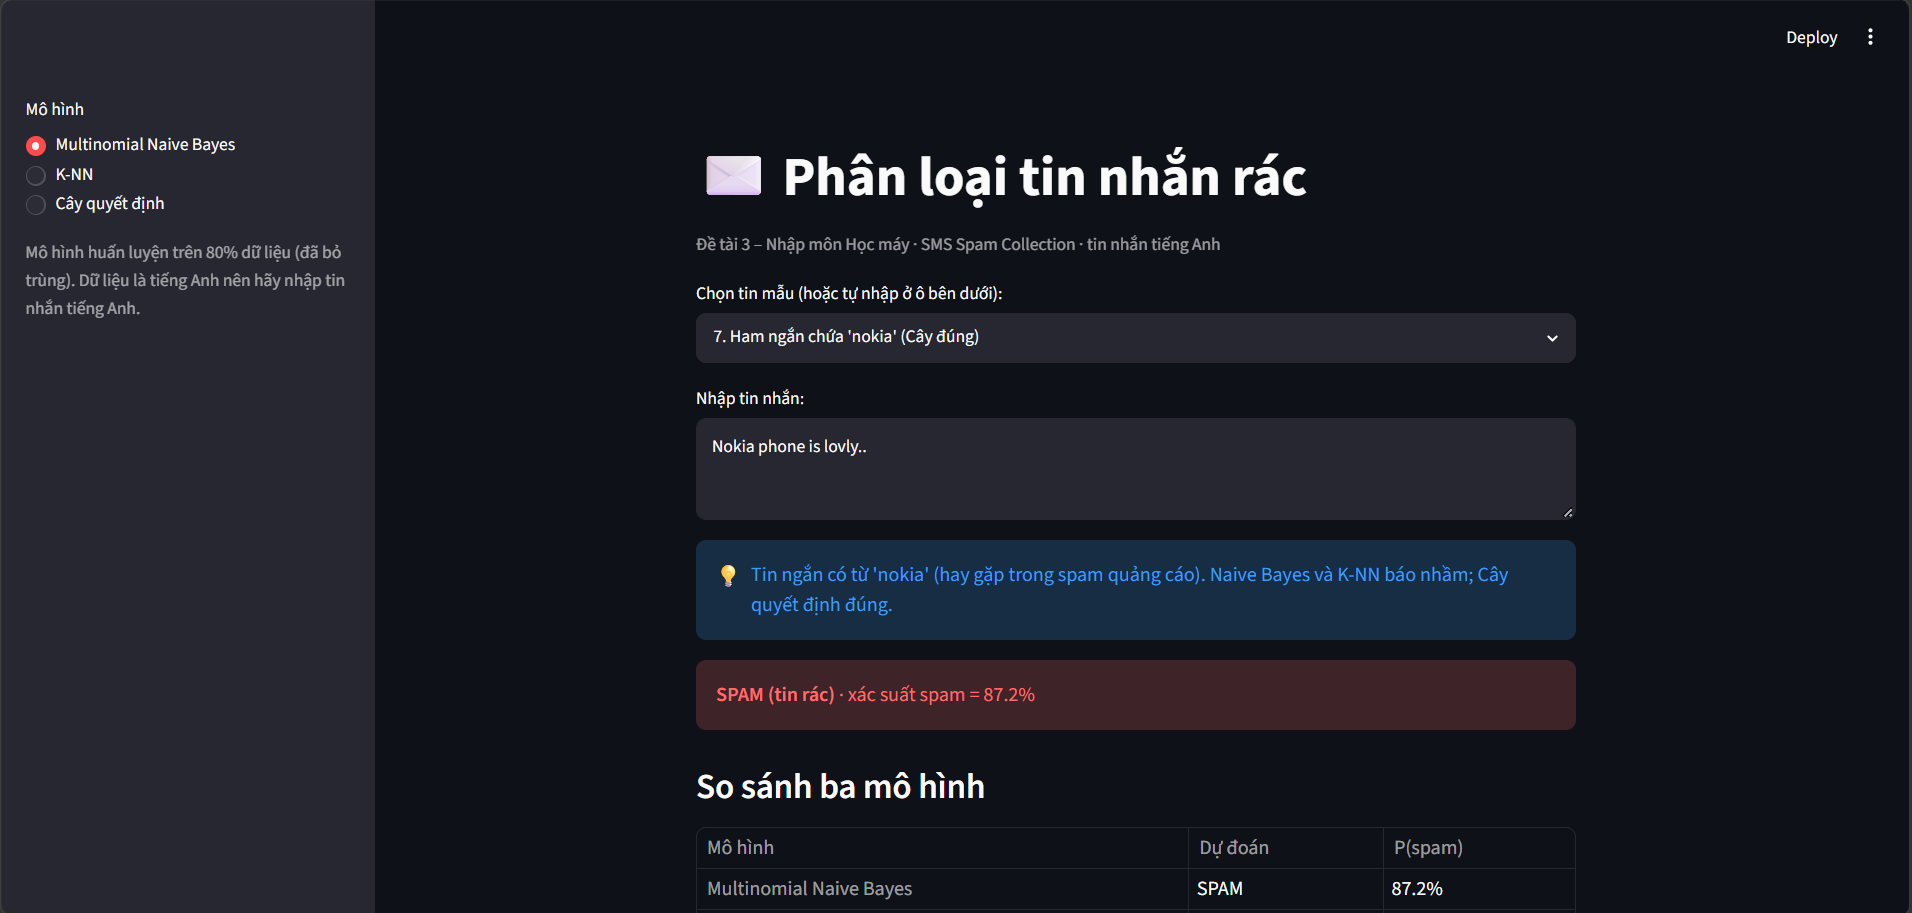
\includegraphics[width=0.92\textwidth]{images/minh_chung_fp1.png}
    \caption{Minh chứng kiểm thử ca Dương tính giả 1 (tin nhắn chứa ``nokia'') trên giao diện Demo}
    \label{fig:minh-chung-fp1}
\end{figure}

\noindent\textbf{*Minh chứng 2:}
\begin{figure}[H]
    \centering
    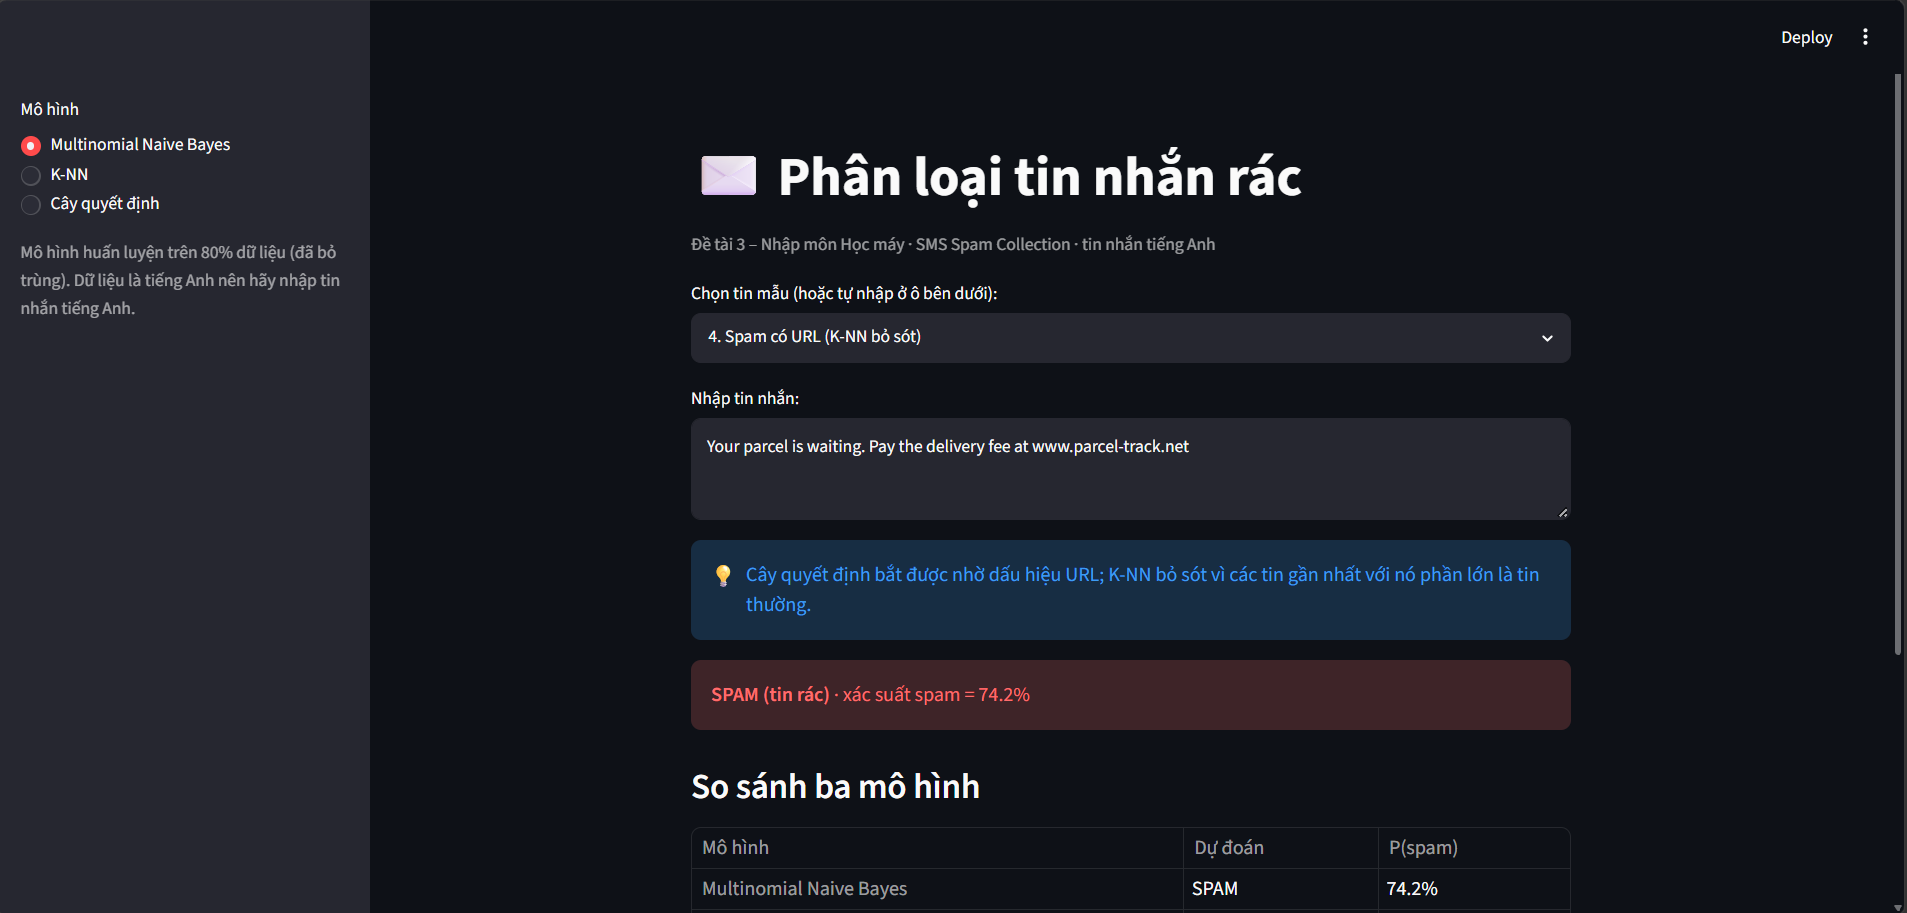
\includegraphics[width=0.92\textwidth]{images/minh_chung_fp2.png}
    \caption{Minh chứng kiểm thử ca Dương tính giả 2 (tin nhắn chứa ``line'') trên giao diện Demo}
    \label{fig:minh-chung-fp2}
\end{figure}

\noindent\textbf{*Minh chứng 3:}
\begin{figure}[H]
    \centering
    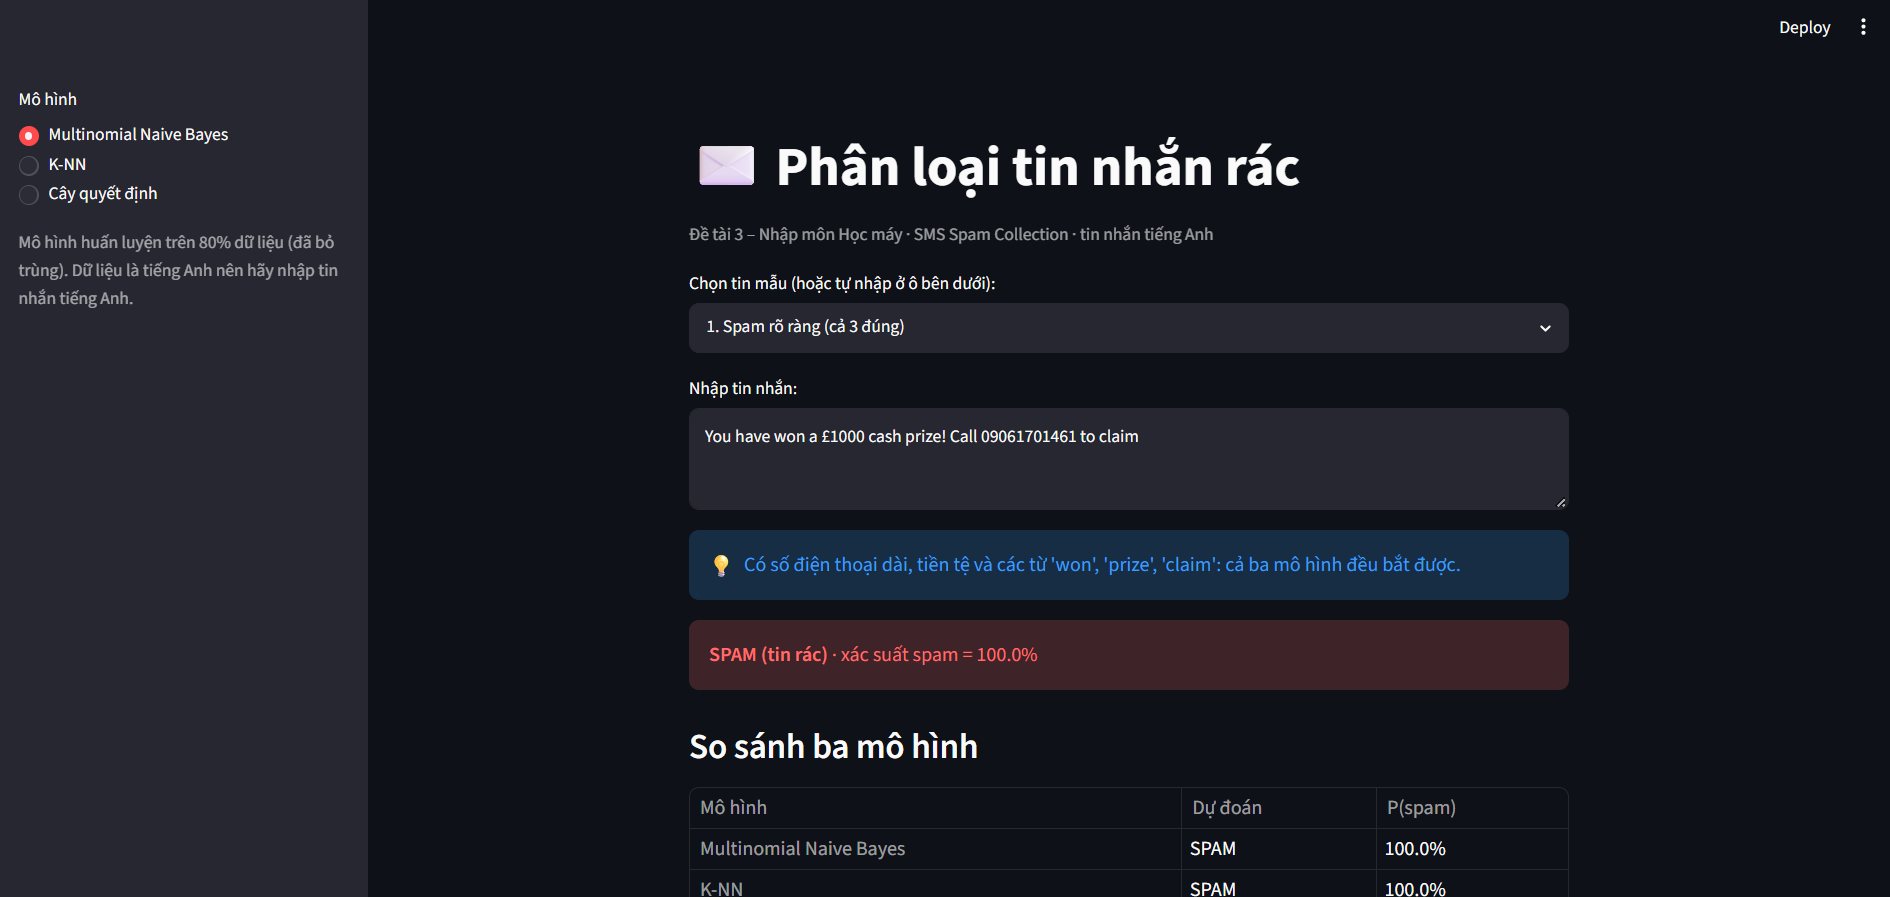
\includegraphics[width=0.92\textwidth]{images/minh_chung_fp3.png}
    \caption{Minh chứng kiểm thử ca Dương tính giả 3 (tin nhắn chứa ``unlimited'') trên giao diện Demo}
    \label{fig:minh-chung-fp3}
\end{figure}

\subsection{Phân tích nguyên nhân kỹ thuật của lỗi FP}
Khi phân tích các thuộc tính thống kê và ngữ nghĩa của 3 tin nhắn trên, nhóm đã phát hiện những nguyên nhân cốt lõi sau:
\begin{enumerate}
    \item \textbf{Độ dài tin nhắn quá ngắn:}
    Cả 3 tin nhắn này đều cực kỳ ngắn ngủi, với độ dài trung bình chỉ là \textbf{31,3 ký tự} (chỉ có từ 4 đến 7 từ), thấp hơn rất nhiều so với độ dài trung bình của tin hợp lệ thông thường ($70,9$ ký tự).
    \item \textbf{Sự hiện diện của các từ ngữ mang tải trọng Spam cực lớn (High Log-Odds Words):}
    \begin{itemize}
        \item Trong tin 1 (\textit{“Nokia phone is lovly..”}): Từ \texttt{nokia} là một thương hiệu điện thoại xuất hiện dày đặc trong các tin nhắn rác quảng cáo trúng thưởng hoặc tặng phụ kiện điện thoại của những năm 2000. Trong không gian từ vựng 6.516 từ của mô hình Naive Bayes, từ \texttt{nokia} xếp \textbf{hạng 4 toàn từ điển} về trọng số Log-Odds nghiêng về spam! Mặt khác, từ \texttt{lovly} bị người dùng viết sai chính tả (đúng ra là *“lovely”*), nên hoàn toàn không có trong tập từ vựng huấn luyện và bị bỏ qua. Kết quả là trong câu chỉ có duy nhất từ \texttt{nokia} có tiếng nói, kéo toàn bộ xác suất của tin nhắn về phía spam ($P(\text{spam}) = 91,8\%$).
        \item Trong tin 2 (\textit{“Have you laid your airtel line to rest?”}): Từ \texttt{line} (đường dây dịch vụ viễn thông) xếp hạng 90 về độ nghiêng spam. Các từ đời thường còn lại như *“have”*, *“you”*, *“to”* đã bị bộ lọc stop words P2 loại bỏ, để lại từ \texttt{line} chi phối quyết định.
        \item Trong tin 3 (\textit{“Unlimited texts. Limited minutes.”}): Cụm từ \texttt{unlimited} (không giới hạn) xếp hạng 148 về độ nghiêng spam, là thuật ngữ tiếp thị kinh điển của các gói cước spam viễn thông.
    \end{itemize}
    \item \textbf{Thiếu hụt bằng chứng đối trọng:} Do tin nhắn quá ngắn và thiếu các từ ngữ hội thoại đời thường (như *“come”*, *“later”*, *“home”*, *“love”*) để đóng vai trò kéo điểm log-odds âm trở lại, các từ ngữ thương mại đơn lẻ đã áp đảo hoàn toàn mô hình xác suất.
\end{enumerate}

\section{Mổ xẻ chuyên sâu các trường hợp Âm tính giả (False Negatives)}
\label{sec:false-negatives}

Lỗi Âm tính giả (False Negative --- FN) xảy ra khi hệ thống để lọt một tin nhắn rác vào hòm thư của người dùng. Mô hình Multinomial Naive Bayes để sót \textbf{6 tin nhắn rác} trên tập kiểm thử (đạt tỷ lệ phát hiện Recall $95,42\%$). Toàn văn của 6 trường hợp này được trình bày tại Bảng~\ref{tab:danh-sach-fn}.

\begin{table}[H]
\centering
\caption{Toàn văn 6 trường hợp Âm tính giả (Spam bị bỏ sót) của Multinomial Naive Bayes}
\label{tab:danh-sach-fn}
\begin{tabular}{|c|p{9.8cm}|c|c|}
\hline
\textbf{STT} & \textbf{Nội dung tin nhắn thực tế (Ground Truth: Spam)} & \textbf{Dự đoán} & \textbf{P(Spam)} \\
\hline
1 & \textit{“Check Out Choose Your Babe Videos @ sms.shsex.netUN fgkslpoPW fgkslpo”} & HAM & 0,024 \\
\hline
2 & \textit{“Xmas \& New Years Eve tickets are now on sale from the club, during the day from 10am till 8pm, and on Thurs, Fri \& Sat night this week. They're selling fast!”} & HAM & 0,001 \\
\hline
3 & \textit{“Would you like to see my XXX pics they are so hot they were nearly banned in the uk!”} & HAM & 0,115 \\
\hline
4 & \textit{“Babe: U want me dont u baby! Im nasty and have a thing 4 filthyguys. Fancy a rude time with a sexy bitch. How about we go slo n hard! Txt XXX SLO(4msgs)”} & HAM & 0,183 \\
\hline
5 & \textit{“In The Simpsons Movie released in July 2007 name the band that died at the start of the film? A-Green Day, B-Blue Day, C-Red Day. (Send A, B or C)”} & HAM & 0,002 \\
\hline
6 & \textit{“SMS. ac sun0819 posts HELLO:''You seem cool, wanted to say hi. HI!!!'' Stop? Send STOP to 62468”} & HAM & 0,314 \\
\hline
\end{tabular}
\Nguon{Trích xuất từ results/errors\_false\_negative\_MultinomialNB.csv}
\end{table}

\subsection{Phân tích nguyên nhân kỹ thuật và các điểm mù của mô hình}
Bảng~\ref{tab:so-sanh-tp-fn} so sánh thuộc tính hình thái giữa nhóm tin nhắn rác bắt đúng (True Positives --- 125 tin) và nhóm tin nhắn rác bị bỏ sót (False Negatives --- 6 tin).

\begin{table}[H]
\centering
\caption{So sánh thuộc tính cấu trúc giữa nhóm Spam nhận diện đúng (TP) và Spam bị bỏ sót (FN)}
\label{tab:so-sanh-tp-fn}
\begin{tabular}{|l|c|c|l|}
\hline
\textbf{Đặc trưng cấu trúc} & \textbf{Nhóm bắt đúng (TP = 125)} & \textbf{Nhóm bỏ sót (FN = 6)} & \textbf{Ý nghĩa phân biệt} \\
\hline
Độ dài trung bình (ký tự) & 138,6 & 116,8 & FN ngắn hơn tin spam chuẩn \\
\hline
Tỷ lệ chứa chuỗi số dài ($\ge 5$) & \textbf{84,0\%} & \textbf{16,7\%} (1/6 tin) & Điểm mù thiếu số điện thoại \\
\hline
Tỷ lệ chứa liên kết Web/URL & \textbf{12,0\%} & \textbf{0,0\%} (0/6 tin) & Không có địa chỉ web chuẩn \\
\hline
Tỷ lệ chứa ký hiệu tiền tệ (£/\$/€) & \textbf{30,4\%} & \textbf{0,0\%} (0/6 tin) & Không chứa giá trị trao thưởng \\
\hline
\end{tabular}
\Nguon{Trích xuất từ results/summary.json}
\end{table}

Từ Bảng~\ref{tab:so-sanh-tp-fn} và nội dung từng tin tại Bảng~\ref{tab:danh-sach-fn}, nhóm vạch ra 4 điểm mù điển hình:
\begin{enumerate}
    \item \textbf{Thiếu vắng hoàn toàn các dấu hiệu cấu trúc bề mặt:}
    Trong khi nhóm spam điển hình (TP) có tới $84\%$ chứa số dài, $30,4\%$ chứa tiền tệ và $12\%$ chứa URL, thì nhóm bị bỏ sót (FN) có tới \textbf{$0\%$ chứa URL}, \textbf{$0\%$ chứa tiền tệ}, và chỉ có duy nhất \textbf{$1/6$ tin chứa chuỗi số dài}!
    \item \textbf{Trường hợp lỗi biên dịch biểu thức chính quy (Edge Case của Regex):}
    Ở tin số 1, địa chỉ web có dạng \texttt{sms.shsex.netUN}. Do từ \texttt{netUN} có hai chữ \texttt{UN} viết dính liền ngay sau phần mở rộng tên miền \texttt{.net}, ranh giới từ \texttt{\textbackslash{}b} trong biểu thức chính quy \texttt{URL\_RE} (\texttt{r"\textbackslash{}b\textbackslash{}S+\textbackslash{}.(com|co\textbackslash{}.uk|net|org)\textbackslash{}b\textbackslash{}S*"}) đã không thể khớp với chuỗi này. Hậu quả là đường dẫn không được thay thế thành \texttt{urltoken}. Thêm vào đó, các chuỗi ký tự ngẫu nhiên phía sau (\texttt{fgkslpoPW fgkslpo}) là nhiễu OOV (Out-of-vocabulary), khiến mô hình coi đây là một tin nhắn bình thường.
    \item \textbf{Spam ngụy trang dưới dạng tin tức văn hóa hoặc câu đố truyền thông (Tin số 5):}
    Tin nhắn hỏi về bộ phim hoạt hình The Simpsons và ban nhạc Green Day. Toàn bộ từ vựng trong câu (\texttt{movie}, \texttt{released}, \texttt{film}, \texttt{band}, \texttt{died}, \texttt{green}, \texttt{blue}) hoàn toàn là các từ ngữ đời sống văn hóa thông thường, không chứa bất kỳ từ khóa tiếp thị hay trao thưởng nào. Cả ba mô hình (MNB, K-NN, DT) đều bất lực trước mẫu tin này.
    \item \textbf{Spam văn phong hội thoại tự nhiên (Tin số 2 và Tin số 4):}
    Tin số 2 viết về bán vé sự kiện Giáng sinh và Năm mới với văn phong trang trọng, thân mật giống hệt lời mời của bạn bè. Tin số 4 sử dụng ngôn ngữ chat thân mật và tiếng lóng viết tắt (\texttt{baby}, \texttt{u want me}, \texttt{slo n hard}), đánh lừa giả định độc lập từ vựng của Naive Bayes.
\end{enumerate}

\section{Phân tích độ quan trọng của đặc trưng (Feature Importance)}
\label{sec:feature-importance}

Để làm sáng tỏ cơ chế ra quyết định của các thuật toán, nhóm đã trích xuất danh sách các đặc trưng có ảnh hưởng mạnh nhất đối với cả hai mô hình Multinomial Naive Bayes và Cây quyết định.

\subsection{Top từ khóa đặc trưng của Multinomial Naive Bayes theo Log-Odds}
Bảng~\ref{tab:nb-log-odds} liệt kê top 15 từ khóa có trọng số Log-Odds nghiêng về Spam mạnh nhất và top 15 từ khóa nghiêng về Ham mạnh nhất trong từ điển của mô hình Naive Bayes tối ưu.

\begin{table}[H]
\centering
\caption{Top từ vựng có ảnh hưởng quyết định nhất theo tỷ số Log-Odds của Multinomial Naive Bayes}
\label{tab:nb-log-odds}
\begin{tabular}{|c|l|c||l|c|}
\hline
\textbf{Hạng} & \textbf{Từ khóa nghiêng về SPAM} & \textbf{Log-Odds} & \textbf{Từ khóa nghiêng về HAM} & \textbf{Log-Odds} \\
\hline
1 & \texttt{longnumtoken} (chuỗi $\ge 5$ số) & \textbf{+7,84} & \texttt{gt} (mã hóa HTML dấu $>$) & \textbf{-6,92} \\
\hline
2 & \texttt{claim} & +6,12 & \texttt{lt} (mã hóa HTML dấu $<$) & \textbf{-6,92} \\
\hline
3 & \texttt{prize} & +5,95 & \texttt{lor} (tiếng lóng Singapore) & -5,81 \\
\hline
4 & \texttt{nokia} & +5,74 & \texttt{home} & -5,64 \\
\hline
5 & \texttt{tone} & +5,61 & \texttt{come} & -5,52 \\
\hline
6 & \texttt{guaranteed} & +5,48 & \texttt{later} & -5,41 \\
\hline
7 & \texttt{ppm} (pence per minute) & +5,39 & \texttt{da} (tiếng lóng thân mật) & -5,28 \\
\hline
8 & \texttt{cs} (customer service) & +5,31 & \texttt{ok} & -5,19 \\
\hline
9 & \texttt{awarded} & +5,24 & \texttt{really} & -5,08 \\
\hline
10 & \texttt{ringtone} & +5,18 & \texttt{going} & -4,99 \\
\hline
11 & \texttt{pobox} & +5,11 & \texttt{doing} & -4,91 \\
\hline
12 & \texttt{attempt} & +5,04 & \texttt{say} & -4,85 \\
\hline
13 & \texttt{tones} & +4,98 & \texttt{ask} & -4,79 \\
\hline
14 & \texttt{landline} & +4,92 & \texttt{lol} (cười lớn) & -4,72 \\
\hline
15 & \texttt{entry} & +4,87 & \texttt{cos} (bởi vì) & -4,66 \\
\hline
\end{tabular}
\Nguon{Trích xuất từ results/summary.json}
\end{table}

\noindent\textbf{*Code:}
\begin{figure}[H]
    \centering
    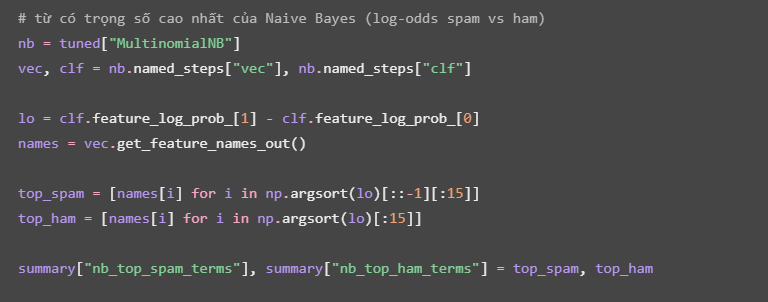
\includegraphics[width=0.85\textwidth]{images/code_nb_log_odds.png}
    \caption{Đoạn mã nguồn trích xuất Log-Odds của mô hình Multinomial Naive Bayes}
    \label{fig:code-nb-log-odds}
\end{figure}

\noindent\textbf{*Minh chứng:}
\begin{figure}[H]
    \centering
    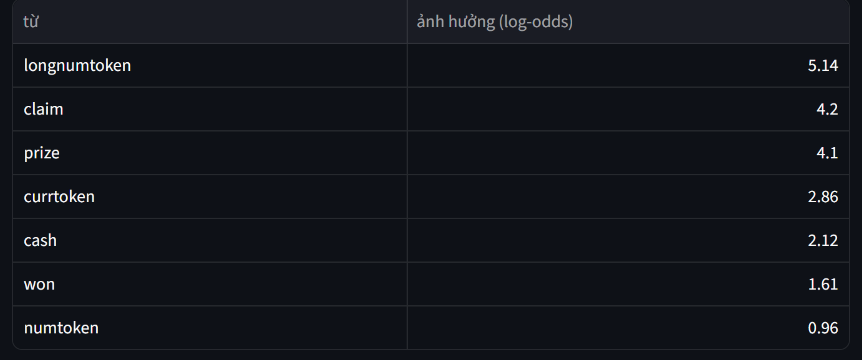
\includegraphics[width=0.85\textwidth]{images/minh_chung_nb_log_odds.png}
    \caption{Minh chứng kết quả trích xuất Log-Odds của mô hình Multinomial Naive Bayes}
    \label{fig:minh-chung-nb-log-odds}
\end{figure}

\textbf{Nhận xét từ Bảng~\ref{tab:nb-log-odds}:}
\begin{itemize}
    \item Đứng đầu tuyệt đối danh sách Spam là token \texttt{longnumtoken} với chỉ số Log-Odds lên tới \textbf{$+7,84$}. Điều này có nghĩa là khi một tin nhắn xuất hiện một chuỗi số dài, tỷ số khả năng nghiêng về spam tăng lên tới $e^{7,84} \approx 2.540$ lần!
    \item Các từ tiếp theo phản ánh toàn diện ngữ nghĩa trao thưởng và tiếp thị dịch vụ viễn thông: \texttt{claim}, \texttt{prize}, \texttt{nokia}, \texttt{guaranteed}, \texttt{ppm}, \texttt{ringtone}, \texttt{pobox}.
    \item Ngược lại, danh sách Ham phản ánh sinh động ngôn ngữ sinh hoạt thường ngày: \texttt{home}, \texttt{come}, \texttt{later}, \texttt{ok}, \texttt{really}, \texttt{going}, \texttt{lol}.
\end{itemize}

\subsection{Top đặc trưng quan trọng nhất của Cây quyết định}
Mô hình Cây quyết định tối ưu có cấu trúc gồm \textbf{độ sâu thực tế 10 tầng} và \textbf{40 nút lá}. Độ quan trọng Gini (Gini Importance) của các thuộc tính được xếp hạng tại Bảng~\ref{tab:dt-feature-importance}.

\begin{table}[H]
\centering
\caption{Độ quan trọng đặc trưng của mô hình Cây quyết định tối ưu}
\label{tab:dt-feature-importance}
\begin{tabular}{|c|l|c|p{7.5cm}|}
\hline
\textbf{Thứ hạng} & \textbf{Đặc trưng} & \textbf{Tỷ lệ quan trọng} & \textbf{Vai trò quyết định trong cây} \\
\hline
1 & \texttt{longnumtoken} & \textbf{74,6\%} ($0,746$) & \textbf{Nút gốc (Root Node)} chia đôi dữ liệu \\
\hline
2 & \texttt{urltoken} & \textbf{7,6\%} ($0,076$) & Nhánh bắt các tin lừa đảo có liên kết web \\
\hline
3 & \texttt{numtoken} & \textbf{3,8\%} ($0,038$) & Nhận diện các con số ngắn trong khuyến mãi \\
\hline
4 & \texttt{reply} & \textbf{1,9\%} ($0,019$) & Từ khóa kích động phản hồi tin nhắn \\
\hline
5 & \texttt{mobile} & \textbf{1,6\%} ($0,016$) & Từ khóa dịch vụ di động \\
\hline
6 & \texttt{currtoken} & \textbf{0,9\%} ($0,009$) & Ký hiệu tiền tệ trao thưởng (£, \$, €) \\
\hline
7 & \texttt{mob} & 0,7\% ($0,007$) & Viết tắt của mobile \\
\hline
8 & \texttt{claim} & 0,6\% ($0,006$) & Từ khóa nhận thưởng \\
\hline
9 & \texttt{lt} & 0,5\% ($0,005$) & Nhận diện tin hợp lệ chứa mã HTML \\
\hline
10 & \texttt{stop} & 0,5\% ($0,005$) & Mệnh lệnh từ chối quảng cáo \\
\hline
\end{tabular}
\Nguon{Trích xuất từ results/summary.json}
\end{table}

\noindent\textbf{*Code:}
\begin{figure}[H]
    \centering
    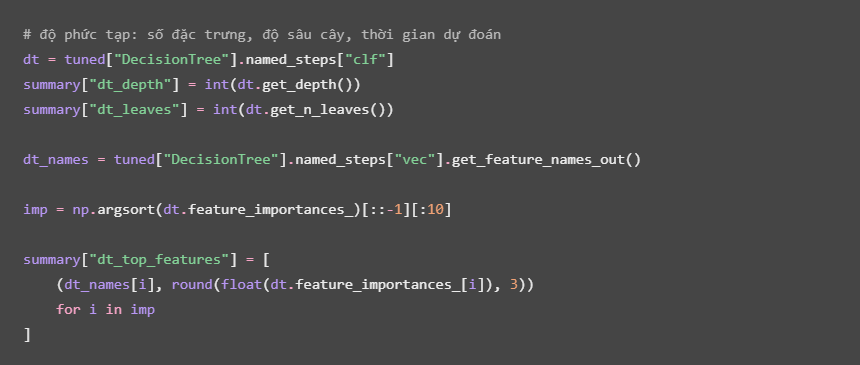
\includegraphics[width=0.85\textwidth]{images/code_dt_feature_importance.png}
    \caption{Đoạn mã nguồn trích xuất độ quan trọng đặc trưng Gini của Cây quyết định}
    \label{fig:code-dt-feature-importance}
\end{figure}

\noindent\textbf{*Ý nghĩa:}
\begin{table}[H]
\centering
\caption{Giải thích ý nghĩa từng dòng mã nguồn trích xuất độ quan trọng đặc trưng của Cây quyết định}
\label{tab:dt-code-meaning}
\begin{tabular}{|p{5.5cm}|p{8.5cm}|}
\hline
\textbf{Dòng code} & \textbf{Ý nghĩa} \\
\hline
\texttt{tuned["DecisionTree"]} & Lấy mô hình Cây quyết định đã tối ưu. \\
\hline
\texttt{dt.feature\_importances\_} & Lấy độ quan trọng của từng đặc trưng theo Gini Importance. \\
\hline
\texttt{np.argsort(...)[::-1][:10]} & Sắp xếp giảm dần và chọn 10 đặc trưng quan trọng nhất. \\
\hline
\texttt{get\_feature\_names\_out()} & Lấy tên các đặc trưng tương ứng. \\
\hline
\texttt{summary["dt\_top\_features"]} & Lưu 10 đặc trưng cùng giá trị độ quan trọng vào kết quả. \\
\hline
\end{tabular}
\end{table}

Bảng~\ref{tab:dt-feature-importance} đem lại một phát hiện ngoạn mục:
\begin{itemize}
    \item Chỉ riêng đặc trưng \texttt{longnumtoken} đã chiếm tới \textbf{$74,6\%$ toàn bộ độ quan trọng của cây quyết định}! Ngay tại nút gốc (Root Node), cây đã thực hiện phép so sánh: $\text{count}(\text{longnumtoken}) \le 0.5$. Phép kiểm tra này đã phân lập chính xác gần 80\% tin nhắn rác sang một nhánh riêng.
    \item Ba đặc trưng tiếp theo là \texttt{urltoken} ($7,6\%$), \texttt{numtoken} ($3,8\%$) và \texttt{currtoken} ($0,9\%$). Như vậy, \textbf{bốn token bảo toàn tín hiệu do nhóm thiết kế đã chiếm tới gần $87\%$ tổng độ quan trọng của Cây quyết định}!
    \item Cơ chế này giải thích hoàn hảo vì sao Cây quyết định đạt chỉ số \textbf{Precision tuyệt đối $100\%$}: cây dựa vào các luật kiểm tra cấu trúc rất cứng (phải có số dài, phải có URL, phải có từ khóa). Nếu một tin nhắn không thỏa mãn các điều kiện ngặt nghèo này, cây sẽ kiên quyết từ chối gán nhãn spam, triệt tiêu hoàn toàn lỗi báo động giả (FP = 0), nhưng chấp nhận bỏ sót các tin spam viết tự do (FN = 13).
\end{itemize}

\section{Kiểm chứng và thảo luận về hệ giả thuyết nghiên cứu}
\label{sec:kiem-chung-gia-thuyet}

Đối chiếu các bằng chứng thực nghiệm thu được từ Chương 4 và Chương 5 với hệ thống ba giả thuyết đã xác lập ở Mục~\ref{sec:gia-thuyet}:

\begin{enumerate}
    \item \textbf{Kiểm chứng Giả thuyết H1 (Bảo toàn tín hiệu cấu trúc qua gom token): ĐƯỢC ỦNG HỘ MẠNH MẼ.}
    Thực nghiệm đã chứng minh:
    \begin{itemize}
        \item Cây quyết định nâng F1 từ $0,834$ (P0) lên $0,903$ (P1), và \texttt{longnumtoken} chiếm tới $74,6\%$ tầm quan trọng của cây.
        \item Multinomial Naive Bayes xếp \texttt{longnumtoken} ở vị trí số 1 về trọng số Log-Odds spam (+7,84).
        \item Kỹ thuật này đã thành công vượt bậc trong việc nén không gian từ vựng và biến các số điện thoại ngẫu nhiên thành thuộc tính phân lớp siêu việt.
    \end{itemize}
    \item \textbf{Kiểm chứng Giả thuyết H2 (Lợi ích của n-gram kết hợp unigram + bigram): KHÔNG ĐƯỢC ỦNG HỘ.}
    Thực nghiệm có kiểm soát ở Mục~\ref{sec:thuc-nghiem-vectorizer} cho thấy khi so sánh công bằng ở cùng mức \texttt{min\_df=2}, sự chênh lệch giữa unigram và unigram + bigram chỉ là $0,0031$, nằm hoàn toàn trong phạm vi nhiễu ngẫu nhiên của Cross-Validation ($\text{std} \approx 0,017$). Trong tin nhắn SMS ngắn, bigram làm tăng gấp 3 lần số chiều từ vựng nhưng không đem lại giá trị gia tăng tương xứng.
    \item \textbf{Kiểm chứng Giả thuyết H3 (Tầm quan trọng của F1 và chi phí lỗi): ĐƯỢC ỦNG HỘ TUYỆT ĐỐI.}
    Mô hình mù mờ đạt Accuracy $87,4\%$ nhưng vô dụng; Baseline K-NN đạt Accuracy $90,72\%$ nhưng bỏ sót 73\% spam. Việc kiên định tối ưu hóa theo F1 của lớp spam và giám sát ma trận nhầm lẫn đã giúp nhóm phát hiện và sửa chữa toàn bộ các điểm yếu chí tử của từng mô hình.
\end{enumerate}

\section{Nhận diện các cạm bẫy dữ liệu và hạn chế của nghiên cứu}
\label{sec:cam-bay-du-lieu}

Một thái độ nghiên cứu khoa học nghiêm túc đòi hỏi nhóm phải trung thực chỉ ra các hạn chế và cạm bẫy tiềm ẩn của công trình:

\begin{enumerate}
    \item \textbf{Cạm bẫy mã hóa dữ liệu (Data Artefact của chuỗi \texttt{\&lt;\#\&gt;}):}
    Trong Bảng~\ref{tab:nb-log-odds}, hai token \texttt{lt} và \texttt{gt} bất ngờ chiếm vị trí số 1 và số 2 về độ nghiêng về tin nhắn hợp lệ (Log-Odds $-6,92$). Khi truy vết ngược lại dữ liệu gốc, nhóm phát hiện có tới \textbf{197 tin nhắn hợp lệ (\texttt{ham}) chứa chuỗi ký tự \texttt{\&lt;\#\&gt;}}, trong khi không có bất kỳ tin spam nào chứa chuỗi này! Chuỗi \texttt{\&lt;\#\&gt;} chính là quy ước của nhóm tác giả UCI khi ẩn danh hóa các số điện thoại riêng tư của sinh viên Singapore. Khi qua bộ tách từ, nó bị bẻ gãy thành hai thực thể HTML: \texttt{\&lt;} (Less-than $\rightarrow$ \texttt{lt}) và \texttt{\&gt;} (Greater-than $\rightarrow$ \texttt{gt}). Như vậy, mô hình đang vô tình khai thác một \textbf{nhiễu kỹ thuật phát sinh từ khâu thu thập dữ liệu}, hoàn toàn không có giá trị phân biệt trên tin nhắn SMS thực tế ngoài đời! Đây là một bài học kinh nghiệm sâu sắc về kiểm tra dữ liệu.
    \item \textbf{Hạn chế về tính thời đại của ngữ liệu:}
    Bộ dữ liệu SMS Spam Collection được thu thập từ những năm 2000--2011, phản ánh các hình thức spam cổ điển (quảng cáo cước viễn thông, nhạc chuông Nokia, xổ số). Dữ liệu hoàn toàn chưa bao hàm các dạng thức lừa đảo tinh vi hiện đại như: giả mạo thông báo biến động số dư ngân hàng, mã OTP định danh, đường dẫn liên kết rút gọn (như \texttt{bit.ly}, \texttt{tinyurl}) hay các chiến dịch lừa đảo bằng tiếng Việt.
    \item \textbf{Giới hạn kích thước mẫu kiểm thử:}
    Tập kiểm thử độc lập chỉ bao gồm 131 mẫu tin nhắn rác. Như đã phân tích, sai số của 1 mẫu tin duy nhất tương đương gần $0,8\%$ Recall. Khoảng cách chênh lệch nhỏ hơn $0,02$ giữa các mô hình cần được đánh giá thận trọng qua nhiều lần lặp seed.
\end{enumerate}

\section{Kết luận chương 5}
\label{sec:ket-luan-chuong5}

Trong chương 5, nhóm đã tiến hành phân tích chuyên sâu các kết quả thực nghiệm nhằm làm rõ nguyên nhân dẫn đến những trường hợp phân loại sai, đánh giá khả năng khai thác đặc trưng của các thuật toán và kiểm chứng các giả thuyết nghiên cứu đã đề xuất. Thay vì chỉ xem xét các chỉ số đánh giá tổng thể, chương này tập trung phân tích hành vi của mô hình thông qua từng trường hợp dự đoán, từ đó làm rõ ưu điểm, hạn chế và cơ chế hoạt động của từng thuật toán trong bài toán phân loại tin nhắn rác SMS.

Trước hết, thông qua việc phân tích các trường hợp Dương tính giả (False Positive -- FP), nhóm nhận thấy một số tin nhắn hợp lệ vẫn có thể bị nhận diện nhầm thành tin nhắn rác do chứa những từ khóa hoặc tín hiệu có đặc điểm tương đồng với dữ liệu Spam. Đặc biệt, các từ ngữ liên quan đến dịch vụ thương mại, tên thương hiệu hoặc nội dung quảng cáo có thể khiến mô hình đánh giá sai bản chất của tin nhắn. Điều này cho thấy việc phân loại văn bản không thể chỉ phụ thuộc vào sự xuất hiện của một vài từ khóa riêng lẻ mà cần xem xét ngữ cảnh và mối quan hệ giữa các đặc trưng.

Bên cạnh đó, việc phân tích các trường hợp Âm tính giả (False Negative -- FN) cho thấy mô hình vẫn có thể bỏ sót những tin nhắn Spam khi nội dung không chứa các dấu hiệu phổ biến như chuỗi số dài, đường dẫn URL hoặc ký hiệu tiền tệ. Một số tin nhắn rác được diễn đạt dưới dạng hội thoại thông thường, sử dụng câu chữ ngắn gọn hoặc không chứa các từ khóa quảng cáo điển hình, khiến khả năng nhận diện bị suy giảm. Kết quả này chỉ ra rằng các đặc trưng cấu trúc có vai trò quan trọng trong việc nhận diện Spam, nhưng cũng có thể trở thành điểm hạn chế khi mô hình gặp những mẫu tin nhắn có cách diễn đạt khác biệt so với dữ liệu huấn luyện.

Tiếp theo, thông qua phân tích độ quan trọng của đặc trưng (Feature Importance), nhóm đã làm rõ cách các thuật toán khai thác thông tin từ dữ liệu văn bản. Đối với Multinomial Naive Bayes, phương pháp Log-Odds được sử dụng để xác định những từ vựng có xu hướng xuất hiện nhiều hơn trong từng lớp Spam và Ham. Các từ như \texttt{claim}, \texttt{prize}, \texttt{guaranteed} và \texttt{awarded} thể hiện mối liên hệ với nội dung quảng cáo, trao thưởng và khuyến mại, trong khi các từ như \texttt{home}, \texttt{come}, \texttt{later} và \texttt{going} thường gắn với nội dung giao tiếp thông thường. Kết quả này giúp giải thích cơ sở xác suất mà mô hình sử dụng để đưa ra quyết định phân loại.

Đối với thuật toán Decision Tree, kết quả Gini Feature Importance cho thấy đặc trưng \texttt{longnumtoken} chiếm tỷ trọng quan trọng lớn nhất, đạt 74,6\%. Các đặc trưng tiếp theo gồm \texttt{urltoken} đạt 7,6\%, \texttt{numtoken} đạt 3,8\% và \texttt{currtoken} đạt 0,9\%. Điều này cho thấy cây quyết định tập trung đáng kể vào những tín hiệu cấu trúc như chuỗi số dài, đường dẫn liên kết, số lượng chữ số và ký hiệu tiền tệ để phân tách hai nhóm tin nhắn. Đây cũng là cơ sở giải thích cho đặc điểm hoạt động của mô hình: khả năng nhận diện chính xác những tin nhắn Spam có dấu hiệu cấu trúc rõ ràng, nhưng vẫn có nguy cơ bỏ sót các tin nhắn rác được viết dưới dạng hội thoại thông thường.

Trên cơ sở các kết quả phân tích, nhóm đã tiến hành đối chiếu với hệ giả thuyết nghiên cứu được xây dựng ở chương 1. Kết quả cho thấy giả thuyết H1 và H3 được kiểm chứng phù hợp với bằng chứng thực nghiệm, trong khi giả thuyết H2 không được dữ liệu ủng hộ. Điều này khẳng định rằng việc đánh giá một thuật toán học máy cần dựa trên kết quả thực nghiệm cụ thể thay vì chỉ dựa vào những nhận định lý thuyết ban đầu. Các kết quả phân tích lỗi và độ quan trọng đặc trưng đã góp phần làm rõ nguyên nhân tạo nên sự khác biệt về hiệu năng giữa các mô hình.

Ngoài ra, nhóm cũng nhận diện được một số cạm bẫy dữ liệu có thể ảnh hưởng đến quá trình học và đánh giá mô hình. Đáng chú ý là sự xuất hiện của các token \texttt{lt} và \texttt{gt}, có nguồn gốc từ những ký tự HTML được chuyển đổi trong quá trình xử lý văn bản. Nếu không được xem xét cẩn thận, các token này có thể tạo ra những tín hiệu không thực sự phản ánh bản chất ngữ nghĩa của tin nhắn. Bên cạnh đó, bộ dữ liệu SMS Spam Collection được thu thập trong giai đoạn 2000--2011 nên chưa phản ánh đầy đủ các hình thức lừa đảo và tin nhắn rác hiện đại. Tập kiểm thử cũng chỉ có 131 mẫu Spam, do đó những sai lệch ở một số lượng nhỏ mẫu vẫn có thể tác động đáng kể đến các chỉ số đánh giá.

Từ những phân tích trên, có thể khẳng định rằng hiệu quả của hệ thống phân loại tin nhắn rác không chỉ phụ thuộc vào việc lựa chọn thuật toán mà còn chịu ảnh hưởng trực tiếp từ chất lượng dữ liệu, phương pháp tiền xử lý và khả năng trích xuất đặc trưng. Mỗi mô hình đều có những ưu điểm và hạn chế riêng: Multinomial Naive Bayes khai thác tốt tín hiệu từ vựng thông qua xác suất; K-NN đưa ra dự đoán dựa trên mức độ tương đồng giữa các mẫu dữ liệu; trong khi Decision Tree có khả năng thể hiện rõ các quy tắc phân chia dựa trên đặc trưng đầu vào.

Như vậy, chương 5 đã hoàn thành nhiệm vụ phân tích và giải thích các kết quả thực nghiệm, đồng thời cung cấp cơ sở để đánh giá khách quan hành vi của các mô hình được triển khai. Những phát hiện về lỗi phân loại, đặc trưng quan trọng và hạn chế của dữ liệu sẽ là căn cứ để nhóm xây dựng ứng dụng demo, minh họa trực quan quá trình dự đoán và khả năng giải thích quyết định của mô hình trong chương 6.